% Section 5. Rewritten 2026-11-03 (branch docs/cep-grounded-draft) from the code as implemented and the rerun in
% docs/optics/rerun_results.md (scripts/rerun_paper_numbers.py). Claim changes: papers/cep/CLAIM_CHANGES.md.
\providecommand{\pending}[1]{\textbf{[PENDING: #1]}}% defined in main.tex; fallback for standalone builds
\section{Crystal detection as implemented}\label{sec:detection}

This section describes the two classical detectors exactly as the code runs them, the size window they apply and the
depth range they admit. Their output is analysed in \secref{sec:csd}; none of it has yet been compared with
hand-labelled crystals (\secref{sec:validation}).

\subsection{Frame conditioning and sharpness layers}\label{sec:layers}

Each frame of the case-study clip is cropped to the live camera picture. The automatic crop of
\code{optics.video_io.resolve_crop} keeps $1826 \times 906$ of the $1920 \times 1080$ clip pixels (80\,\%); the
single-frame figures use the fixed crop of $1800 \times 905$~px (79\,\%). At the modelled scale of \secref{sec:budget}
($1.464 \times 1.913$~\umpx{} at focus; $\pm\,{\approx}10$\,\% input budget, not validated in the image) the
automatic crop covers
${\approx}\,2.7 \times 1.7$~mm of slurry.

A per-pixel sharpness map is computed as the logarithm of the squared Laplacian smoothed by a $15 \times 15$~px
Gaussian (\code{annotator.sharpness}). A depth score combines the min--max-normalised inverse sharpness (weight 0.7)
with the normalised Farneb\"ack optical-flow magnitude to the previous sampled frame (weight 0.3; zero for a single
frame). The score is quantised uniformly into $L = 3$ layers, and each detector runs once per layer
(\figref{fig:detection} colours detections by layer). The layers order pixels by sharpness and motion; they are not depth measurements, because a
sharpness value maps to two depths (\secref{sec:ambiguity}).

\subsection{Edge and watershed detectors}\label{sec:edge}

Both detectors start from the same Gaussian adaptive threshold (block 11~px, offset 2), which marks the dark crystal
outlines on the bright background.

\emph{Edge detector} (\code{annotator.detection}). The outline map is closed morphologically with an elliptical
kernel of $3 + 4\ell$~px for layer $\ell$; external contours are fitted with minimum-area rotated rectangles, and a
contour is kept if its area lies in the size window (\secref{sec:window}) and its aspect ratio is at most~3.

\emph{Watershed detector} (\code{optics.detect_watershed}). The outline map is opened with a $3 \times 3$ kernel and
its complement is distance-transformed. Seeds are the h-maxima ($h = 2.5$~px) of the distance map that lie at least
6~px from any outline and at least 12~px from each other (\tabref{tab:ws-constants}). A marker-controlled watershed
on the negative distance map, a standard image-segmentation method~\citep{Vincent1991,BeucherMeyer1993}, grows one
basin per seed; each basin is fitted and filtered as above, with the basin pixel count as its area.

\begin{table}
\centering\tabfont
\caption{Seed constants of the watershed detector (CHOICE, module constants of \texttt{optics.detect\_watershed}). The
\textmu m values use the modelled 1080p clip scale of \secref{sec:budget}.}\label{tab:ws-constants}
\begin{tabular}{@{}lr>{\raggedright\arraybackslash}p{0.5\columnwidth}@{}}
\toprule
Constant & Value & Role \\
\midrule
\code{_PEAK_MIN_DISTANCE} & 12~px & minimum seed spacing; $17.6 \times 23.0$~\um{} ($x \times y$) \\
\code{_PEAK_THRESHOLD_ABS} & 6~px & minimum distance of a seed from any outline \\
\code{_H_MAXIMA_PARAM} & 2.5~px & h-maxima height; suppresses plateau peaks \\
\bottomrule
\end{tabular}
\end{table}

A detection's size is the geometric mean $\sqrt{w h}$ of its rectangle sides, converted with the geometric-mean
pixel scale ($1.673$~\umpx{} on the clips). Because a pixel is not square (\secref{sec:chain}), this
area-equivalent size is exact under the anisotropic scale, whereas a chord length in a given direction is not: a
pixel spans 1.464~\um{} along a row and 1.913~\um{} down a column, $-12$\,\% and $+14$\,\% of the geometric mean.

\subsection{Size window from the configuration}\label{sec:window}

The area window is read from \code{configs/camera_100.toml} by \code{optics.config.detection_area_px}. Its lower
bound is $3^2 = 9$~px$^2$ (\code{min_side_px} $= 3$, CHOICE). Its upper bound is the pixel area of a 1~mm square at
the focused plane, $\mathit{max\_size}^2 / (\mu_x \mu_y)$ with the per-axis scales $\mu_x, \mu_y$; the 1~mm
(\code{max_size_um}, CHOICE) rounds up the 0.821~mm largest crystal of the first microscope reading
(\secref{sec:expected}). On the 1080p clips the window is $[9,\ 356\,474]$~px$^2$, an area-equivalent 5--1000~\um;
on the PAL recording it is $[9,\ 71\,020]$~px$^2$. Three clip pixels are $4.4 \times 5.7$~\um{} but only
${\approx}\,1.1$ PAL samples, because the clips are upscaled PAL pictures; on PAL, three samples are
$11.8 \times 10.8$~\um.

The earlier fixed window $[80,\ 8000]$~px$^2$ corresponds on the clips to an area-equivalent 15--150~\um{}
(13--131~\um{} along a row, 17--171~\um{} down a column). It is reported below only to show how the detector output
depends on the window.

\begin{figure}
\centering
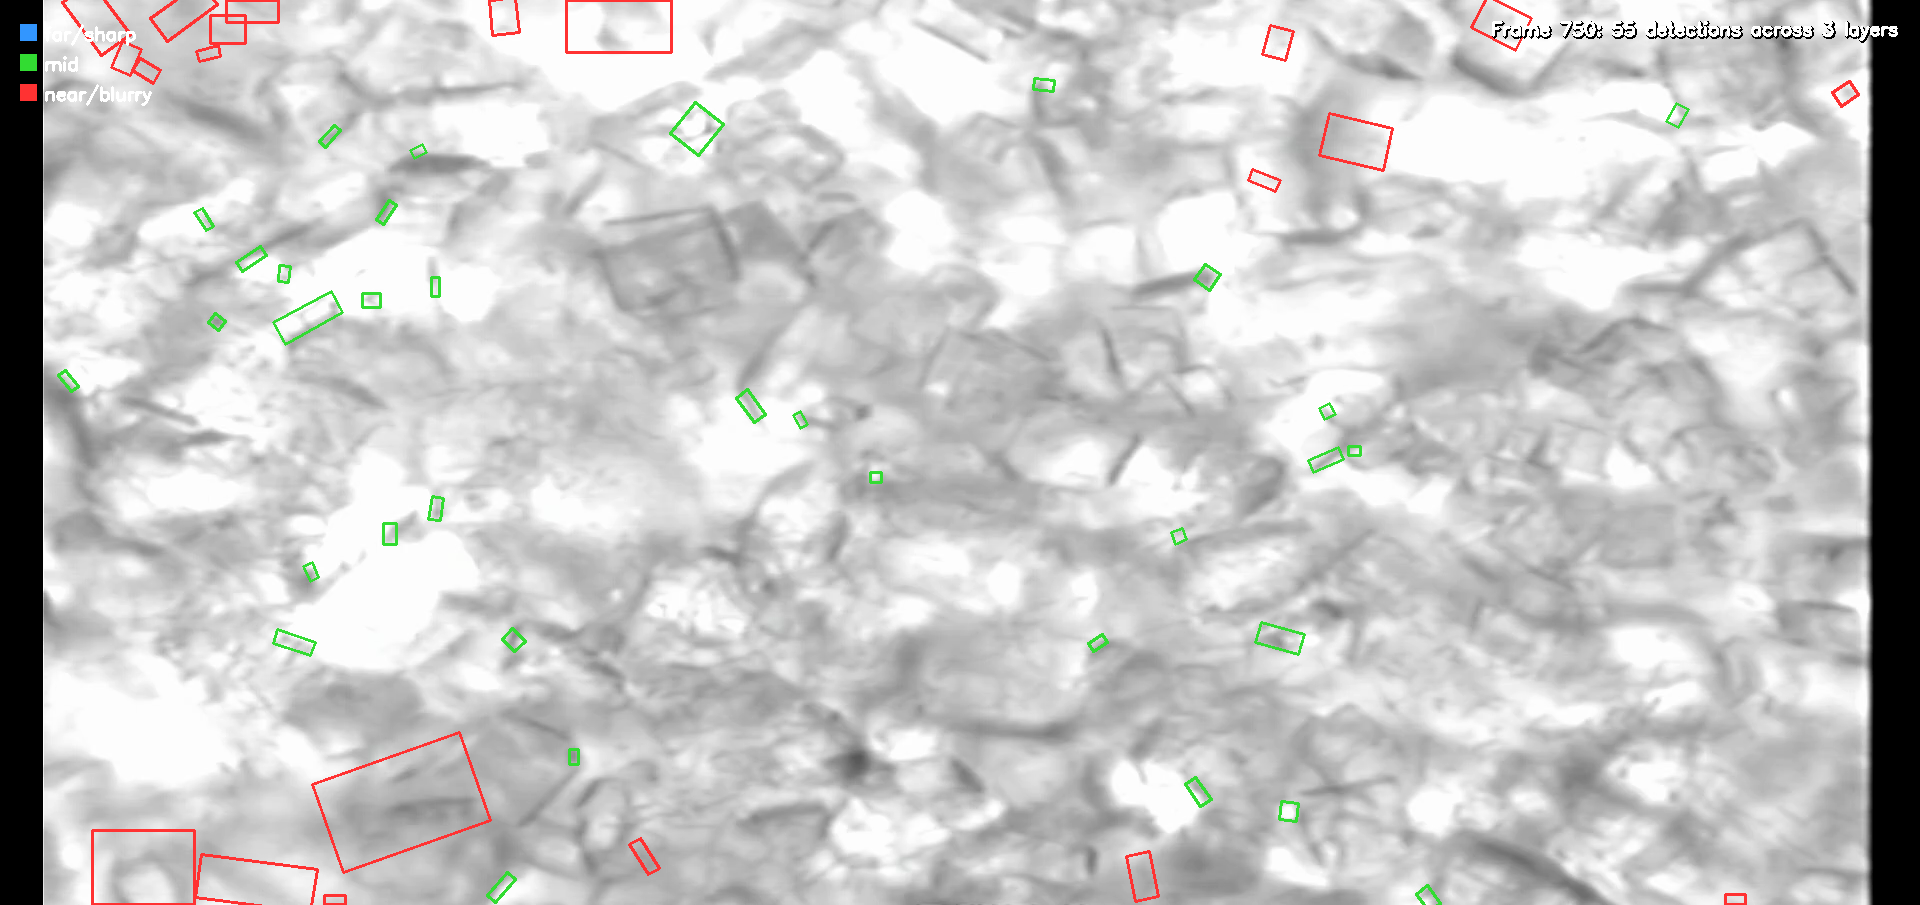
\includegraphics[width=\columnwidth]{11_detection_overlay}
\caption{Edge-detector output on frame 750 with the configured window (\texttt{optics.qualitative}): 840 rotated
rectangles, coloured by sharpness layer (the legend names are the code's layer names, not depth assignments). By
visual reading, not checked against labels, many of the largest rectangles enclose blurred regions rather than single
crystal outlines. The earlier $[80, 8000]$~px$^2$
window gives 292 detections on the same frame.}\label{fig:detection}
\end{figure}

\subsection{Depth range admitted by the detectors}\label{sec:selectivity}

Both detectors need dark outlines a few pixels wide, so they admit only crystals near the focused plane. The
resolution element of the recording is the PAL sample ($6.83 \times 6.25$~\um{} at the sensor, geometric mean
6.53~\um; \secref{sec:chain}), not the upscaled clip pixel. If a detector loses an outline once the circle of
confusion exceeds five resolution elements (an assumption, not a measured threshold), the F/1.6 lens admits
$\delta = \pm 47$~\um{} around focus (\secref{sec:coc}). Over that range the near/far apparent-size ratio of
\eqref{eq:ratio} departs from one by only 0.17\,\%, whereas a 5\,\% difference requires $\delta \approx 1.3$~mm
(\figref{fig:discrim}). Counting in clip pixels instead gives $\pm 21$~\um{} and 0.08\,\%. The size signal that
\secref{sec:sizing} relies on is therefore negligible for any detection these detectors can make at F/1.6.

\begin{figure}
\centering
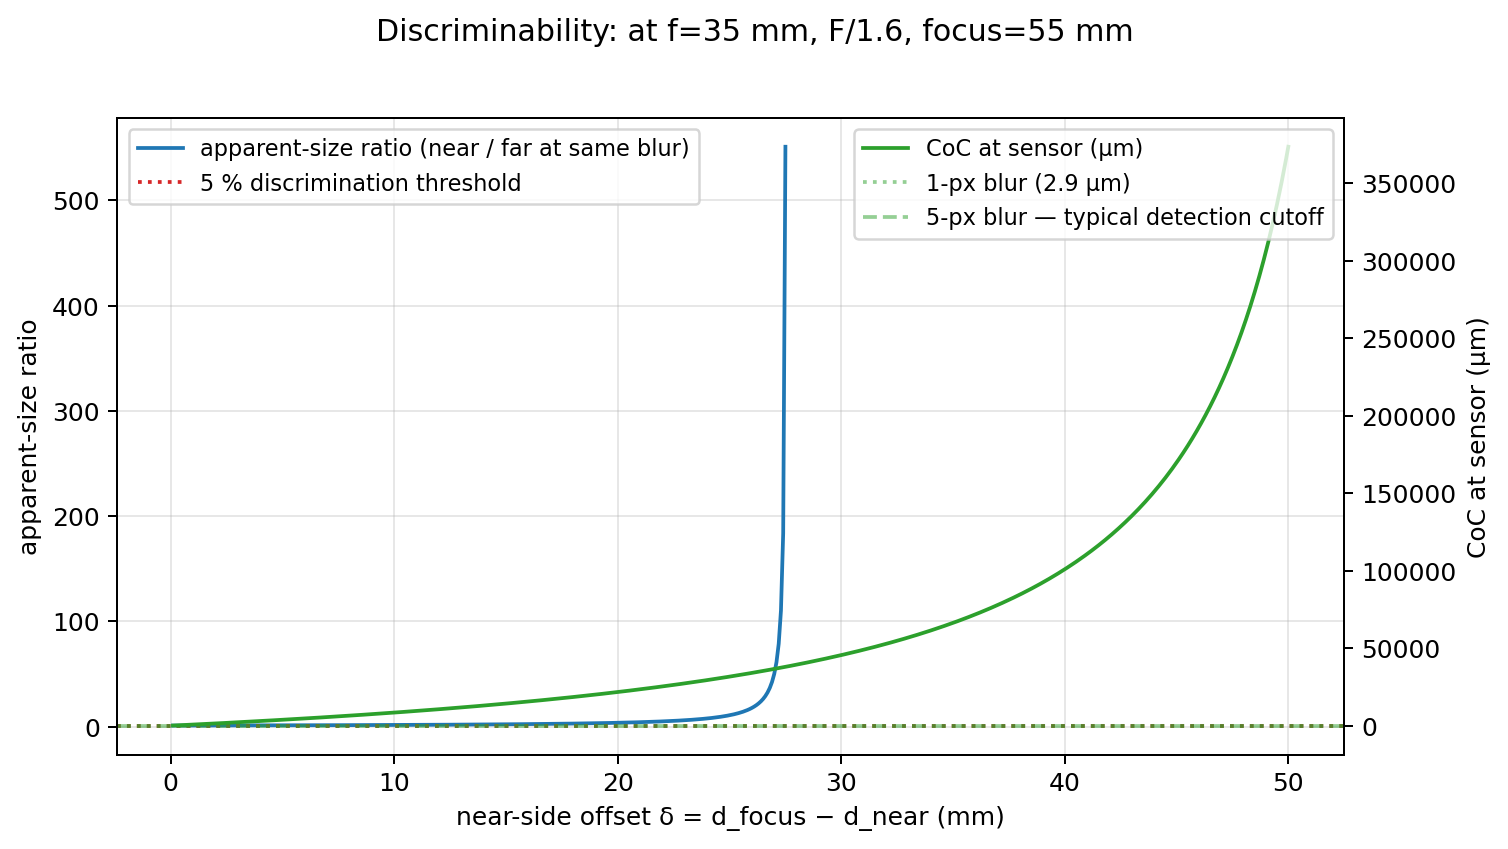
\includegraphics[width=\columnwidth]{10_discriminability}
\caption{Near/far apparent-size difference $d_\mathrm{far}/d_\mathrm{near} - 1$ against the near-side offset
$\delta$ at F/1.6, log axes (\texttt{optics.disambiguate.fig\_discriminability}); the top axis gives the sensor CoC
in PAL samples (6.53~\um). Solid line: in-focus half-slice, 9.4~\um{} (CoC = 1 sample). Dashed: the assumed
five-sample detection cutoff, 47~\um, where the difference is 0.17\,\%. Dotted: 5\,\%, reached at
$\delta \approx 1.3$~mm.}\label{fig:discrim}
\end{figure}
